\documentclass[10pt]{standalone}
\usepackage{amsmath}
\usepackage{amssymb}
\usepackage{pgf,tikz}
\usepackage{mathrsfs}
\usetikzlibrary{arrows}
\pagestyle{empty}
\usepackage{siunitx}
\begin{document}
	

	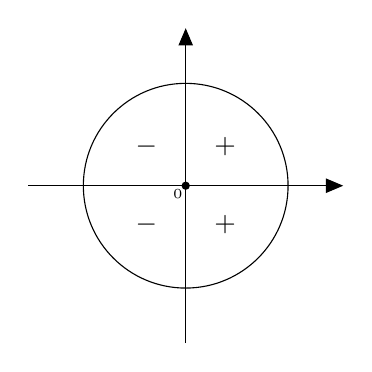
\begin{tikzpicture}[>=triangle 45]
	\draw[->,color=black] (-2,0) -- (2,0);
	\draw[->,color=black] (0,-2) -- (0,2);
	\draw(0,0) circle (1.3);
	\node (a1) at (-0.5,0.5)  {$\mathbf{-}$};
	\node(a1) at (0.5,0.5) {$\mathbf{+}$};
	\node(a1) at(-0.5,-0.5 )  {$\mathbf{-}$};
	\node(a1) at (0.5,-0.5)  {$\mathbf{+}$};
	
	\fill [color=black] (0,0) circle (1.5pt);
		\draw (-0.1,-0.1) node {{\tiny \ensuremath{0}}};
	\end{tikzpicture}
\end{document}